% arara: xelatex

\documentclass[12pt]{article} % размер шрифта

\usepackage{etex} % extend
\usepackage{tikz} % картинки в tikz
\usepackage{microtype} % свешивание пунктуации

\usepackage{diagbox}
\usepackage{slashbox}
\usepackage{tabularx}
\usepackage{comment}

\usepackage{tikzlings}
\usepackage{tikzducks}

\usepackage{array} % для столбцов фиксированной ширины
\usepackage{verbatim} % для вставки комментариев

\usepackage{indentfirst} % отступ в первом параграфе

\usepackage{sectsty} % для центрирования названий частей

\allsectionsfont{\centering} % приказываем центрировать все sections

\usepackage{amsmath,  amsfonts} % куча стандартных математических плюшек

\usepackage[top=1.5cm,  left=1.5cm,  right=1.5cm,  bottom=1.5cm]{geometry} % размер текста на странице

\usepackage{lastpage} % чтобы узнать номер последней страницы

\usepackage{enumitem} % дополнительные плюшки для списков
%  например \begin{enumerate}[resume] позволяет продолжить нумерацию в новом списке
\usepackage{caption} % подписи к картинкам без плавающего окружения figure

\usepackage{comment} % длинные комментарии

\usepackage{fancyhdr} % весёлые колонтитулы
\pagestyle{fancy}
\lhead{Теория вероятностей и статистика,  НИУ-ВШЭ}
\rhead{Домашняя работа}
\chead{}
\cfoot{}
\rfoot{}
\renewcommand{\headrulewidth}{0.4pt}
\renewcommand{\footrulewidth}{0.4pt}

\usepackage{physics}

\usepackage{todonotes} % для вставки в документ заметок о том,  что осталось сделать
% \todo{Здесь надо коэффициенты исправить}
% \missingfigure{Здесь будет картина Последний день Помпеи}
% команда \listoftodos — печатает все поставленные \todo'шки

\usepackage{booktabs} % красивые таблицы
% заповеди из документации:
% 1. Не используйте вертикальные линии
% 2. Не используйте двойные линии
% 3. Единицы измерения помещайте в шапку таблицы
% 4. Не сокращайте .1 вместо 0.1
% 5. Повторяющееся значение повторяйте,  а не говорите "то же"

\usepackage{fontspec} % поддержка разных шрифтов
\usepackage{polyglossia} % поддержка разных языков

\setmainlanguage{russian}
\setotherlanguages{english}

\setmainfont{Linux Libertine O} % выбираем шрифт

% можно также попробовать Helvetica,  Arial,  Cambria и т.Д.

% чтобы использовать шрифт Linux Libertine на личном компе, 
% его надо предварительно скачать по ссылке
% http://www.linuxlibertine.org/index.php?id=91&L=1

\newfontfamily{\cyrillicfonttt}{Linux Libertine O}
% пояснение зачем нужно шаманство с \newfontfamily
% http://tex.stackexchange.com/questions/91507/

\AddEnumerateCounter{\asbuk}{\russian@alph}{щ} % для списков с русскими буквами
\setlist[enumerate,  2]{label=\asbuk*), ref=\asbuk*} % списки уровня 2 будут буквами а) б) \ldots 

%% эконометрические и вероятностные сокращения
\DeclareMathOperator{\Cov}{Cov}
\DeclareMathOperator{\Corr}{Corr}
\DeclareMathOperator{\Var}{Var}
\DeclareMathOperator{\E}{\mathbb{E}}
\DeclareMathOperator{\D}{Var}
\newcommand \hb{\hat{\beta}}
\newcommand \hs{\hat{\sigma}}
\newcommand \htheta{\hat{\theta}}
\newcommand \s{\sigma}
\newcommand \hy{\hat{y}}
\newcommand \hY{\hat{Y}}
\newcommand \e{\varepsilon}
\newcommand \he{\hat{\e}}
\newcommand \hVar{\widehat{\Var}}
\newcommand \hCorr{\widehat{\Corr}}
\newcommand \hCov{\widehat{\Cov}}
\newcommand \cN{\mathcal{N}}
\newcommand{\R}{\mathbb{R}}



\let\P\relax
\DeclareMathOperator{\P}{\mathbb{P}}

%\fbox{
%  \begin{minipage}{24em}
%    Фамилия,  имя и номер группы (печатными буквами):\vspace*{3ex}\par
%    \noindent\dotfill\vspace{2mm}
%  \end{minipage}
%  \begin{tabular}{@{}l p{0.8cm} p{0.8cm} p{0.8cm} p{0.8cm} p{0.8cm}@{}}
% %\toprule
% Задача & 1 & 2 & 3 & 4 & 5\\ 
% \midrule
% Балл  &  &  & & & \\
% \midrule
% %\bottomrule
% \end{tabular}
% }    


\begin{document}

\begin{enumerate}
    \item Величина $X$ распределена нормально $\cN(0;\sigma^2)$.
    \begin{enumerate}
        \item Найдите $\E(\abs{X})$.
        \item Найдите функцию плотности $\abs{X}$.
        \item Представьте себе, что вы видите только значения $X$, большие 1. 
        Найдите функцию плотности наблюдаемой случайной величины и вычислите её математическое ожидание. 
    \end{enumerate}


    \item Пёс Шарик и Кот Матроскин каждый день в течение месяца покупают молоко в розлив. 
    Цена молока в $i$-ый день — константа $m_i$. 
    Средняя цена молока за прошедший месяц оказалась равной 40 рублям. 
    Пёс Шарик каждый день покупал литр молока. Кот Матроскин каждый день покупал молока на 40 рублей. 
    
    \begin{enumerate}
        \item Кто больше потратил денег? 
        \item Кто больше молока купил?
    \end{enumerate}
    
    \item Кот Матроскин забрасывает удочку 10 раз.
  Вероятность поймать рыбку при одном забрасывании равна $p$.
  Пёс Шарик забрасывает удочку случайное пуассоновское количество раз,
  $N$, под настроение. Известно, что $\E(N) = 10$.
  
  У кого шансы поймать хотя бы одну рыбку выше?
  
  \item Случайным образом на сфере $x^2+y^2+z^2=1$ равномерно выбирается точка. 
  Её координаты — случайные величины $X$, $Y$ и $Z$.
  
  \begin{enumerate}
      \item Найдите функцию плотности величины $X$.
      \item Найдите совместную функцию плотности пары величин $X$ и $Y$.
      \item Найдите ковариацию величин $X$ и $Y$.
  \end{enumerate}

  \item Компания кабельного телевидения НВТ, Новая Вершина Телевидения, анализирует возможность
  присоединения к своей сети пригородов N-ска. Опросы показали, что в среднем каждые 3 из 12
  семей жителей пригородов хотели бы стать абонентами сети. Стоимость работ, необходимых для
  организации сети в любом пригороде оценивается величиной 2 000 000 у.е. При подключении каждого
  пригорода НВТ надеется получить 1 000 000 у.е. в год от рекламодателей. Планируемая чистая прибыль
  от оплаты за кабельное телевидение одной семьей в год равна 120 у.е.
  
  Каким должно быть минимальное количество семей в пригороде для того, чтобы с вероятностью 0.95
  расходы на организацию сети в этом пригороде окупились за год?
  
  
  \item  Неправильный кубик выпадает с вероятностью $0.5$ шестеркой вверх. 
  Остальные пять граней выпадают равновероятно. 
  Случайная величина $X$ — остаток от деления номера грани на два, 
  $Y$ — остаток от деления номера грани на три. 
 \begin{enumerate}
 \item Найдите закон распределения $\E(X\mid Y)$, $\E(Y\mid X)$.
 \item Выразите $\E(Y\mid X)$ через $X$, а $\E(X\mid Y)$ через $Y$.
 \item Найдите $\Cov(\E(Y\mid X),\E(X\mid Y))$, $\Cov(\E(Y\mid X),X)$, $\Cov(Y,X)$.
 \end{enumerate}
 
    
  \item  Величины $X_1$, \ldots, $X_n$ независимы и одинаково распределены с математическим ожиданием $10$ и дисперсией $20$. 
  Найдите примерный закон распределения величин $\bar X^2$, $(1+\bar{X})/(\bar{X}^2+5)$ при большом $n$.
 \newpage
 \item $ $ \\ % грязный хак!
 \vspace{\baselineskip}
 \begin{minipage}{\linewidth}
 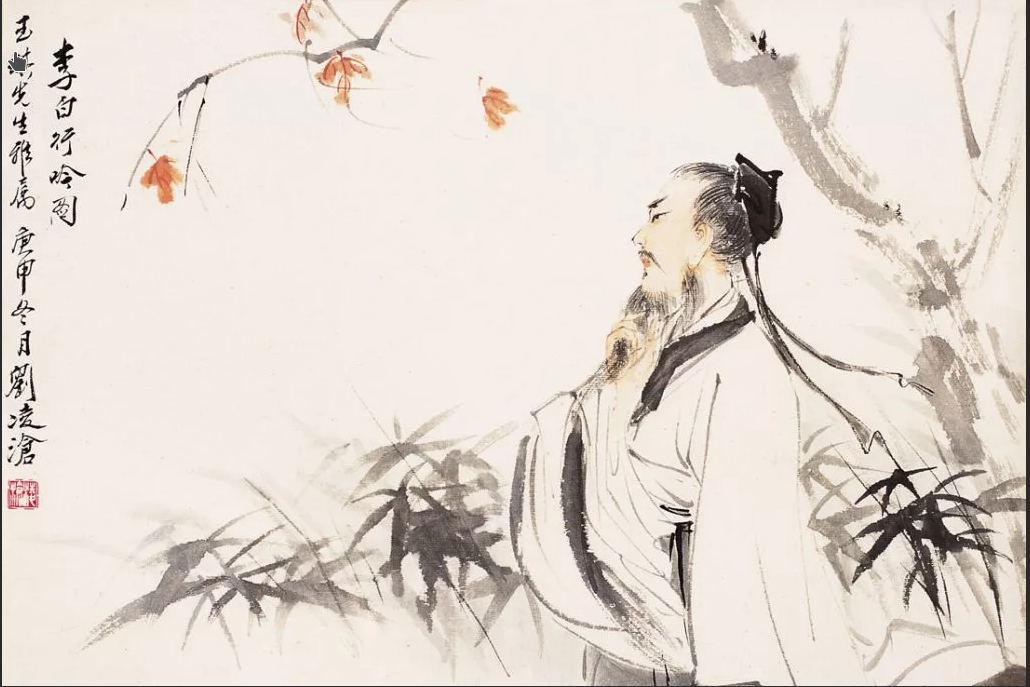
\includegraphics[width=17cm]{libo.png}
 \end{minipage}

 \begin{minipage}{12cm}
 \begin{quote}
    Протрезвел я в цветах, а вокруг уже ночь, \\
    Лепестков облетевших одежда полна. \\
    Вдоль ручья побреду я куда-нибудь прочь, \\
    Где ни птиц, ни людей, только в небе луна. 
    
    \hspace{7cm} \textit{Ли Бо}
    
  \end{quote}
\end{minipage} 
 
\vspace{0.3cm}

    Бессмертный гений поэзии Ли Бо очнулся в случайной равномерно распределенной точке круглой поляны радиусом в один ли. 
    В центре поляны находится розовый куст. 
    \begin{enumerate}
        \item Найдите функцию плотности расстояния от Ли Бо до розового куста в ли. 
        \item Найдите математическое ожидание и дисперсию этого расстояния.
    \end{enumerate}


\end{enumerate}


\end{document}